% \knuthc  knuth the TeXBook
% \lvoc   Lvovsky
% \lamc  lamport latex 
% \slshape different font for footnote
\graphicspath{{sec01/images/s2/}{sec01/code/s2/}}
\lstset{inputpath=sec01/code/s2/}

\begin{frame}[fragile]{How good it will be if...\only<2,3>{we could write like this}}\relax
\begin{center}
\only<1>{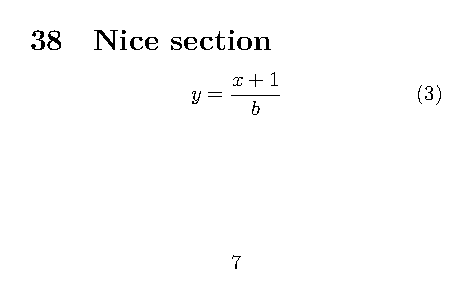
\includegraphics{refBegin}}
\only<2>{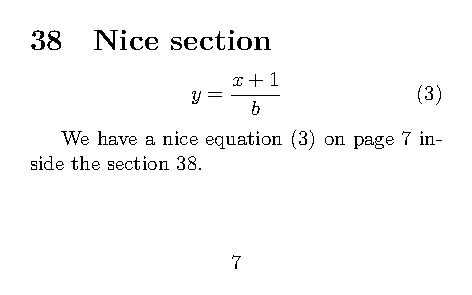
\includegraphics{refBegin2}}
\only<3>{\Huge We can!}
\end{center}

\cprotect\skfootnote{I use \verb|\only<2>{text}| for such effect. Also \verb|\setcounter| was used in source.}
\end{frame}

\begin{frame}[fragile]{Step 1: \ccol\label}\relax
     \lstinputlisting[linerange={12-15}, basicstyle=\tt]{refBegin2.tex}
     
     \skfootnote{for whole reference mechanism: \lmanc{7}[51] \lvoc{I.2.11}[27] \overC{https://www.overleaf.com/learn/latex/Cross_referencing_sections_and_equations}, \wikiC{https://en.wikibooks.org/wiki/LaTeX/Labels_and_Cross-referencing}}
\end{frame}

\begin{frame}[fragile]{Step 2: \ccol{\ref} and \ccol{\pageref}}
     \lstinputlisting[linerange={17-17}, basicstyle=\tt]{refBegin2.tex}
\end{frame}

\begin{frame}[fragile]{Problem 1: lots of labels!}
    What if you have a lot of labels?
    \inclass{\incPause Look throw whole document and compare \TeX\ and pdf?\incPause }
    
\cprotect\twocolImg{
    \lstinputlisting[linerange={10-10, 13-16}, basicstyle=\tt\small]{refBeginShow.tex}
}{refBeginShow}    
    
    
    \skfootnote{\url{http://ctan.altspu.ru/macros/latex/contrib/showlabels/showlabels.pdf}}
\end{frame}

\begin{frame}[fragile]{Problem 2: Typos}\relax
\cprotect\twocolImg{
    \lstinputlisting[linerange={12-17}, basicstyle=\tt\small]{refBad.tex}
}{refBad}           
\end{frame}

\begin{frame}[fragile]{Bibliography}{How to cite}\relax
Use \ccol{\cite\{label\}}

\cprotect\twocolImg{
    \lstinputlisting[linerange={9-9}, basicstyle=\tt\small]{citeFirst.tex}
}{citeFirst}  

\incPause
\cprotect\twocolImg{
    \lstinputlisting[linerange={11-12}, basicstyle=\tt\small]{citeSecond.tex}
}{citeSecond}  

\skfootnote{\lmanc{8.24.2}[94] \wikiC{https://en.wikibooks.org/wiki/LaTeX/Bibliography_Management} \overC{https://www.overleaf.com/learn/latex/Bibliography_management_in_LaTeX}}     
\end{frame}

\begin{frame}[fragile]{Bibliography}{What to cite}\relax

{\csk .bib} files

\begin{verbatim}
@Book{landau,
    author = {Landau, L. D. and Lifshitz, E. M.},
    title = {The Classical Theory of Fields},
    journal = N,
    volume = {1},
    pages = {140},
    year = 1980
}
\end{verbatim}

You can have multiple records in one .bib file.
     
\end{frame}

\begin{frame}[fragile]{Bibliography. Where can you get .bib files?\preMagicPage}\relax
\begin{itemize}
    \item Just google it! ``article\_name bibtex''
    \item Go to you favorite journal and look at Citations -> ``.bib'' or ``bibtex''
    \item Ask Mendeley or other programs to give you the .bib file
    \item Create it by yourself
\end{itemize}
\end{frame}

\begin{frame}[fragile]{Bibliography. Creating .bib file \magicPage}\relax
\begin{center}
\begin{tabular}{rl}
     \ccol{@article} & Journal or magazine article\\
\ccol{@book} & Book\\
\ccol{@conference} & Article in conference proceedings\\
\ccol{@misc} & If nothing else fits.
\end{tabular}
\end{center}
\skfootnote{\wikiC{https://en.wikibooks.org/wiki/LaTeX/Bibliography_Management\#Standard_templates} for cite url checkout \stExC{https://tex.stackexchange.com/questions/3587/how-can-i-use-bibtex-to-cite-a-web-page}
}     
\end{frame}

\begin{frame}[fragile]{Bibliography. Creating .bib file \magicPage}\relax
\begin{center}
{\obeylines
author
title
journal
year
pages
volume
...
}
\end{center}
\skfootnote{check for full list \wikiC{https://en.wikibooks.org/wiki/LaTeX/Bibliography_Management\#BibTeX}
}     
\end{frame}

\begin{frame}[fragile]{Bibliography. Offline\preMagicPage}\relax
Running \LaTeX\ offline, you can get \textbf{(??)} in \ccol{\ref} and \textbf{[?]} in \ccol{\cite}. 

For 
\begin{itemize}
    \item References 
    \item Bibliography
    \item Table of content
    \item Indexing
    \item ...
\end{itemize}

\LaTeX\ collect addition data in extra files. \LaTeX\ need more then one run to get this data. 

Use \verb|latex; bibtex; latex; latex|

\end{frame}

\begin{frame}[fragile]{Bibliography. Manually\magicPage}

You can add Bibliography manually.

\cprotect\twocolImg{
    \lstinputlisting[linerange={10-22}]{citeMan.tex}
}{citeMan}  

\skfootnote{\lmanc{8.24}[92]}
\end{frame}

\begin{frame}[fragile]{Bibliography. Styles\magicPage}

You can change styles.

Mannually -- check \url{https://en.wikibooks.org/wiki/LaTeX/Bibliography_Management}

Our with packages -- check \url{https://tex.stackexchange.com/questions/25701/bibtex-vs-biber-and-biblatex-vs-natbib}
\end{frame}

\begin{frame}[fragile]{Subject index\magicPage}\relax
\cprotect\twocolImg{
    \lstinputlisting[linerange={9-16}]{indexmy.tex}
}{indexmy}  

\skfootnote{\lvoc{IV.7}[175] \lmanc{25.2}[215]}     
\end{frame}